\documentclass[../main.tex]{subfiles}
\graphicspath{{\subfix{../images/}}}
\begin{document}
We say that a random variable X distributes Pareto, denoting $X\sim \text{Par}(x_m,\alpha)$, if the distribution function of X is 
\[f_X(x):= \begin{cases} \frac{\alpha x_m^{\alpha}}{x^{\alpha+1}}, & x\geq x_m \\ 0, & \text{Otherwise} \end{cases}\]
\begin{enumerate}
    
    \item Sample $n=1,000$ samples from a pareto distribution with $x_m=5,\alpha=7$. Show a histogram of these samplings. 
    
    \item Write a function that calculates the likelihood of a single sampling for $x_m=5$ and an unknown $\alpha$. Use this to calculate the general log likelihood of the whole sampling.
    
    \item Numerically find the maximum log-likelihood.
    
    \item Go over this process 10,000 times and find confidence intervals with significance $0.99,0.95$. Show a diagram with 100 confidence intervals with significance $0.95$, and compare to the real parameter value. Discuss the result. 
    
    \item Set $\alpha=1.1$ (leave $x_m$ as is). Estimate numerically the expected value using 100 sampling of sizes 
    \[N\in\{1, 1,00, 10,000, 1,000,000, 100,000,000\} = \{10^0, 10^2, 10^4, 10^6, 10^8\}\]
    Present the results of these 500 samplings. Do the same with $\alpha = 0.9$. Discuss this result
\end{enumerate}

\noindent\line(1,0){480}
\subsection*{Solution:}
The code we are going to use was submitted in an ipynb (jupyter notebook) file. The file supports LaTeX but it isn't easily readable. Therefore we also submit a PDF or .html version of the notebook where it will be easier to read, especially the mathematical parts. Here we will summarize the main results/concepts that we want to present from the code file. 
\begin{enumerate}
    \item In the code file we presented 2 different methods for sampling the pareto distributions. The plots you get from the samplings look like this -

\begin{figure}[H]
\centering
\subcaptionbox{Method Of Sampling "By Hand"}{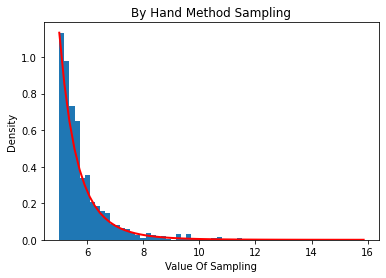
\includegraphics[width=0.46\textwidth]{images/ByHandMethod.png}}%
\hfill % <-- Seperation
\subcaptionbox{Using The Built-In Numpy Function }{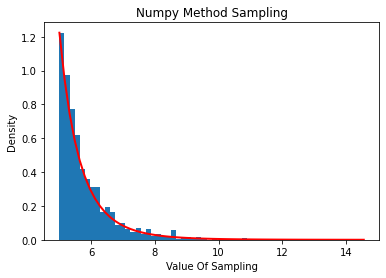
\includegraphics[width=0.46\textwidth]{images/Numpy.png}}%
\caption{Both Sampling Methods}
\end{figure}

Where the red line is the real density function of the distribution, And the blue rectangles are the bins of the histogram of the sampling we got. From these images alone it can be seen that these methods are equivalent (in the sense that both sample from the same distribution). \qedsymbol

\item The solution is fully presented in the code file. Mostly straight-forward and simple code. As an example of this calculation the log-likelihood of the sampling we did using the numpy method. One of the times this came out to be $-767.504510428529$. Of course you can check the notebook that we submitted for the result from the last time it ran before we gave in the project. \qedsymbol

\item We use 2 methods to find the maximum. One numerically (as was asked for), and one analytically. The numerical method uses the gradient descent method (which is described in the jupyter notebook) for the negative log-likelihood (which maximizes our original function), and the analytical solution uses deriving the function and comparing it to 0. We then compare these different solutions. When running the code it can be very quickly seen that these methods lead to \emph{very} close values of $\alpha$. We get the following plot of the log-likelihood and we can see how close our solution is to the real value - 

\begin{mdframed}[backgroundcolor=blue!20] 
    \begin{center}
        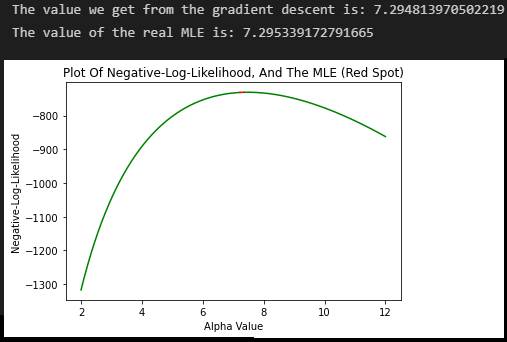
\includegraphics[scale=0.7]{images/Plot And Values.png}
    \end{center}
\end{mdframed}
\item We presented 2 methods in the code. One is based on using MLE-s: if we sample enough MLE-s we can take a confidence interval for the MLE-s which will also serve as a confidence interval for the "real" $\alpha$. The other is based on using pivots. For the pivot we use the following quantity 
\[2\alpha\sum_{i=1}^n \log\left(\frac{x}{x_m}\right)\sim\chi_{2n}^2\]
In the code file there is an explanation for why this is true. We also present a comparison between these methods according to some basic metrics on the intervals - the average length of the intervals, the standard deviation and how much these intervals are symmetric according to the real $\alpha$. 

We then presented 100 confidence intervals according to the pivot method: The intervals are the colorful horizontal lines presented in the following image. The Vertical black line represents the real value of $\alpha$ (in this case $\alpha=7$). The red markers on the side denote which intervals \emph{do not} contain the real $\alpha$ value. We can see that about 5 of the intervals do not contain 7. (When running the code sometimes we get more sometimes we get less). The y-values in the plot are meaningless of course. 
\begin{mdframed}[backgroundcolor=blue!20] 
    \begin{center}
        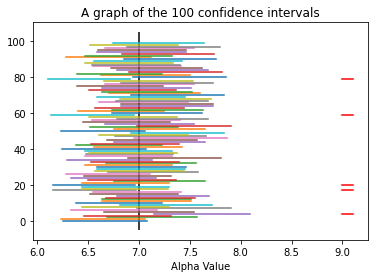
\includegraphics[scale=0.75]{images/10signintrvls.png}
    \end{center}
\end{mdframed}
When looking at the metrics mentioned above we get the following results - 
\begin{mdframed}[backgroundcolor=blue!20] 
    \begin{center}
        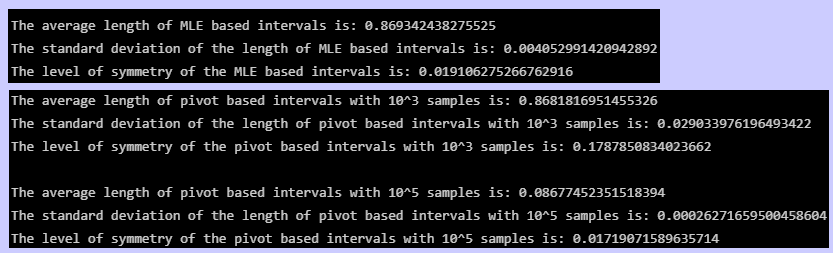
\includegraphics[scale=0.65]{images/Metrics For Different Methods.png}
    \end{center}
\end{mdframed}
Initially this might imply that the MLE method is better than the pivot method because these metrics for the MLE method are equal to or better than the ones for the pivot method for the sample size of $10^3$. The reason this is incorrect is because for the MLE method you need to sample $10^3$ samples $10^4$ times in order to get slightly better metrics than the pivot method with $10^3$ samples, and if we even sample "only" $10^5$ then the pivot method reaches significantly better results. This means the MLE method is much slower to calculate (running this in the code file we sent will show that), and since we can also sample many less samples for the pivot method there are memory advantages to the pivot method. All together this means the pivot method is better. 

\item As is discussed in the code we use the sample average to estimate the mean of the sampling. The plots we got from the code are the following -

\begin{figure}[H]
\centering
\subcaptionbox{\hlfancy{goodcolor}{$\alpha=0.9$}}{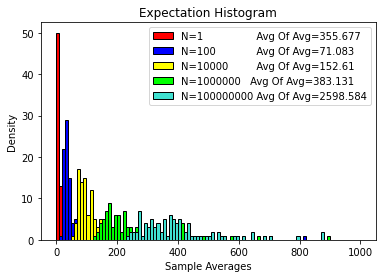
\includegraphics[width=0.46\textwidth]{images/alpha0.9.png}}%
\hfill % <-- Seperation
\subcaptionbox{\hlfancy{goodcolor}{$\alpha=1.1$}}{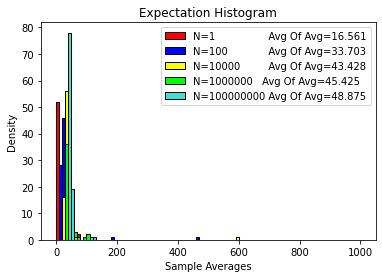
\includegraphics[width=0.46\textwidth]{images/alpha1.1.png}}%
\caption{Histograms of sample averages for $\alpha=0.9/1.1$}
\end{figure}

In the code file we present an explanation for why these results vary so much even though the $\alpha$ values are, at least to the human eye, pretty close. The explanation we provide for this is firstly based on understanding why in general the sample average is an estimate for the mean. Then there is a detailed explanation for why this is problematic for these values - for $\alpha=0.9$ it doesn't work at all, and for $\alpha=1.1$ it works but it's convergence doesn't "feel" very quick (where the suggested explanation considers the fact that the variance of the sampling is infinite). And so we get the obvious divergence between how the sample averages change between our $\alpha$ values. \qedsymbol

\end{enumerate}
\end{document}